\section{Modellierung} % (fold)
\label{sec:modellierung}

\subsection{Ereignisgesteuerte Prozessketten} % (fold)
\label{sub:ereignisgesteuerte_prozessketten}

Aus der Aufgabenbeschreibung ergeben sich die in Abbildung~\ref{fig:epk} dargestellten \ac{EPK} für Erzeuger und Verbraucher. Hierbei ist zu erkennen, dass sich die Prozesse bei identischem Ablaufschema lediglich in den  durchgeführten Prüfungen und Operationen unterscheiden. Hierdurch liegt es nahe, dass die Ablaufsteuerung im objektorientierten Entwurf in einer abstrakten Basisklasse modelliert wird, und nur die unterschiedlichen Handlungen in den jeweiligen spezialisierten Ableitungen konkretisiert werden.

\begin{figure}[H]
\begin{center}
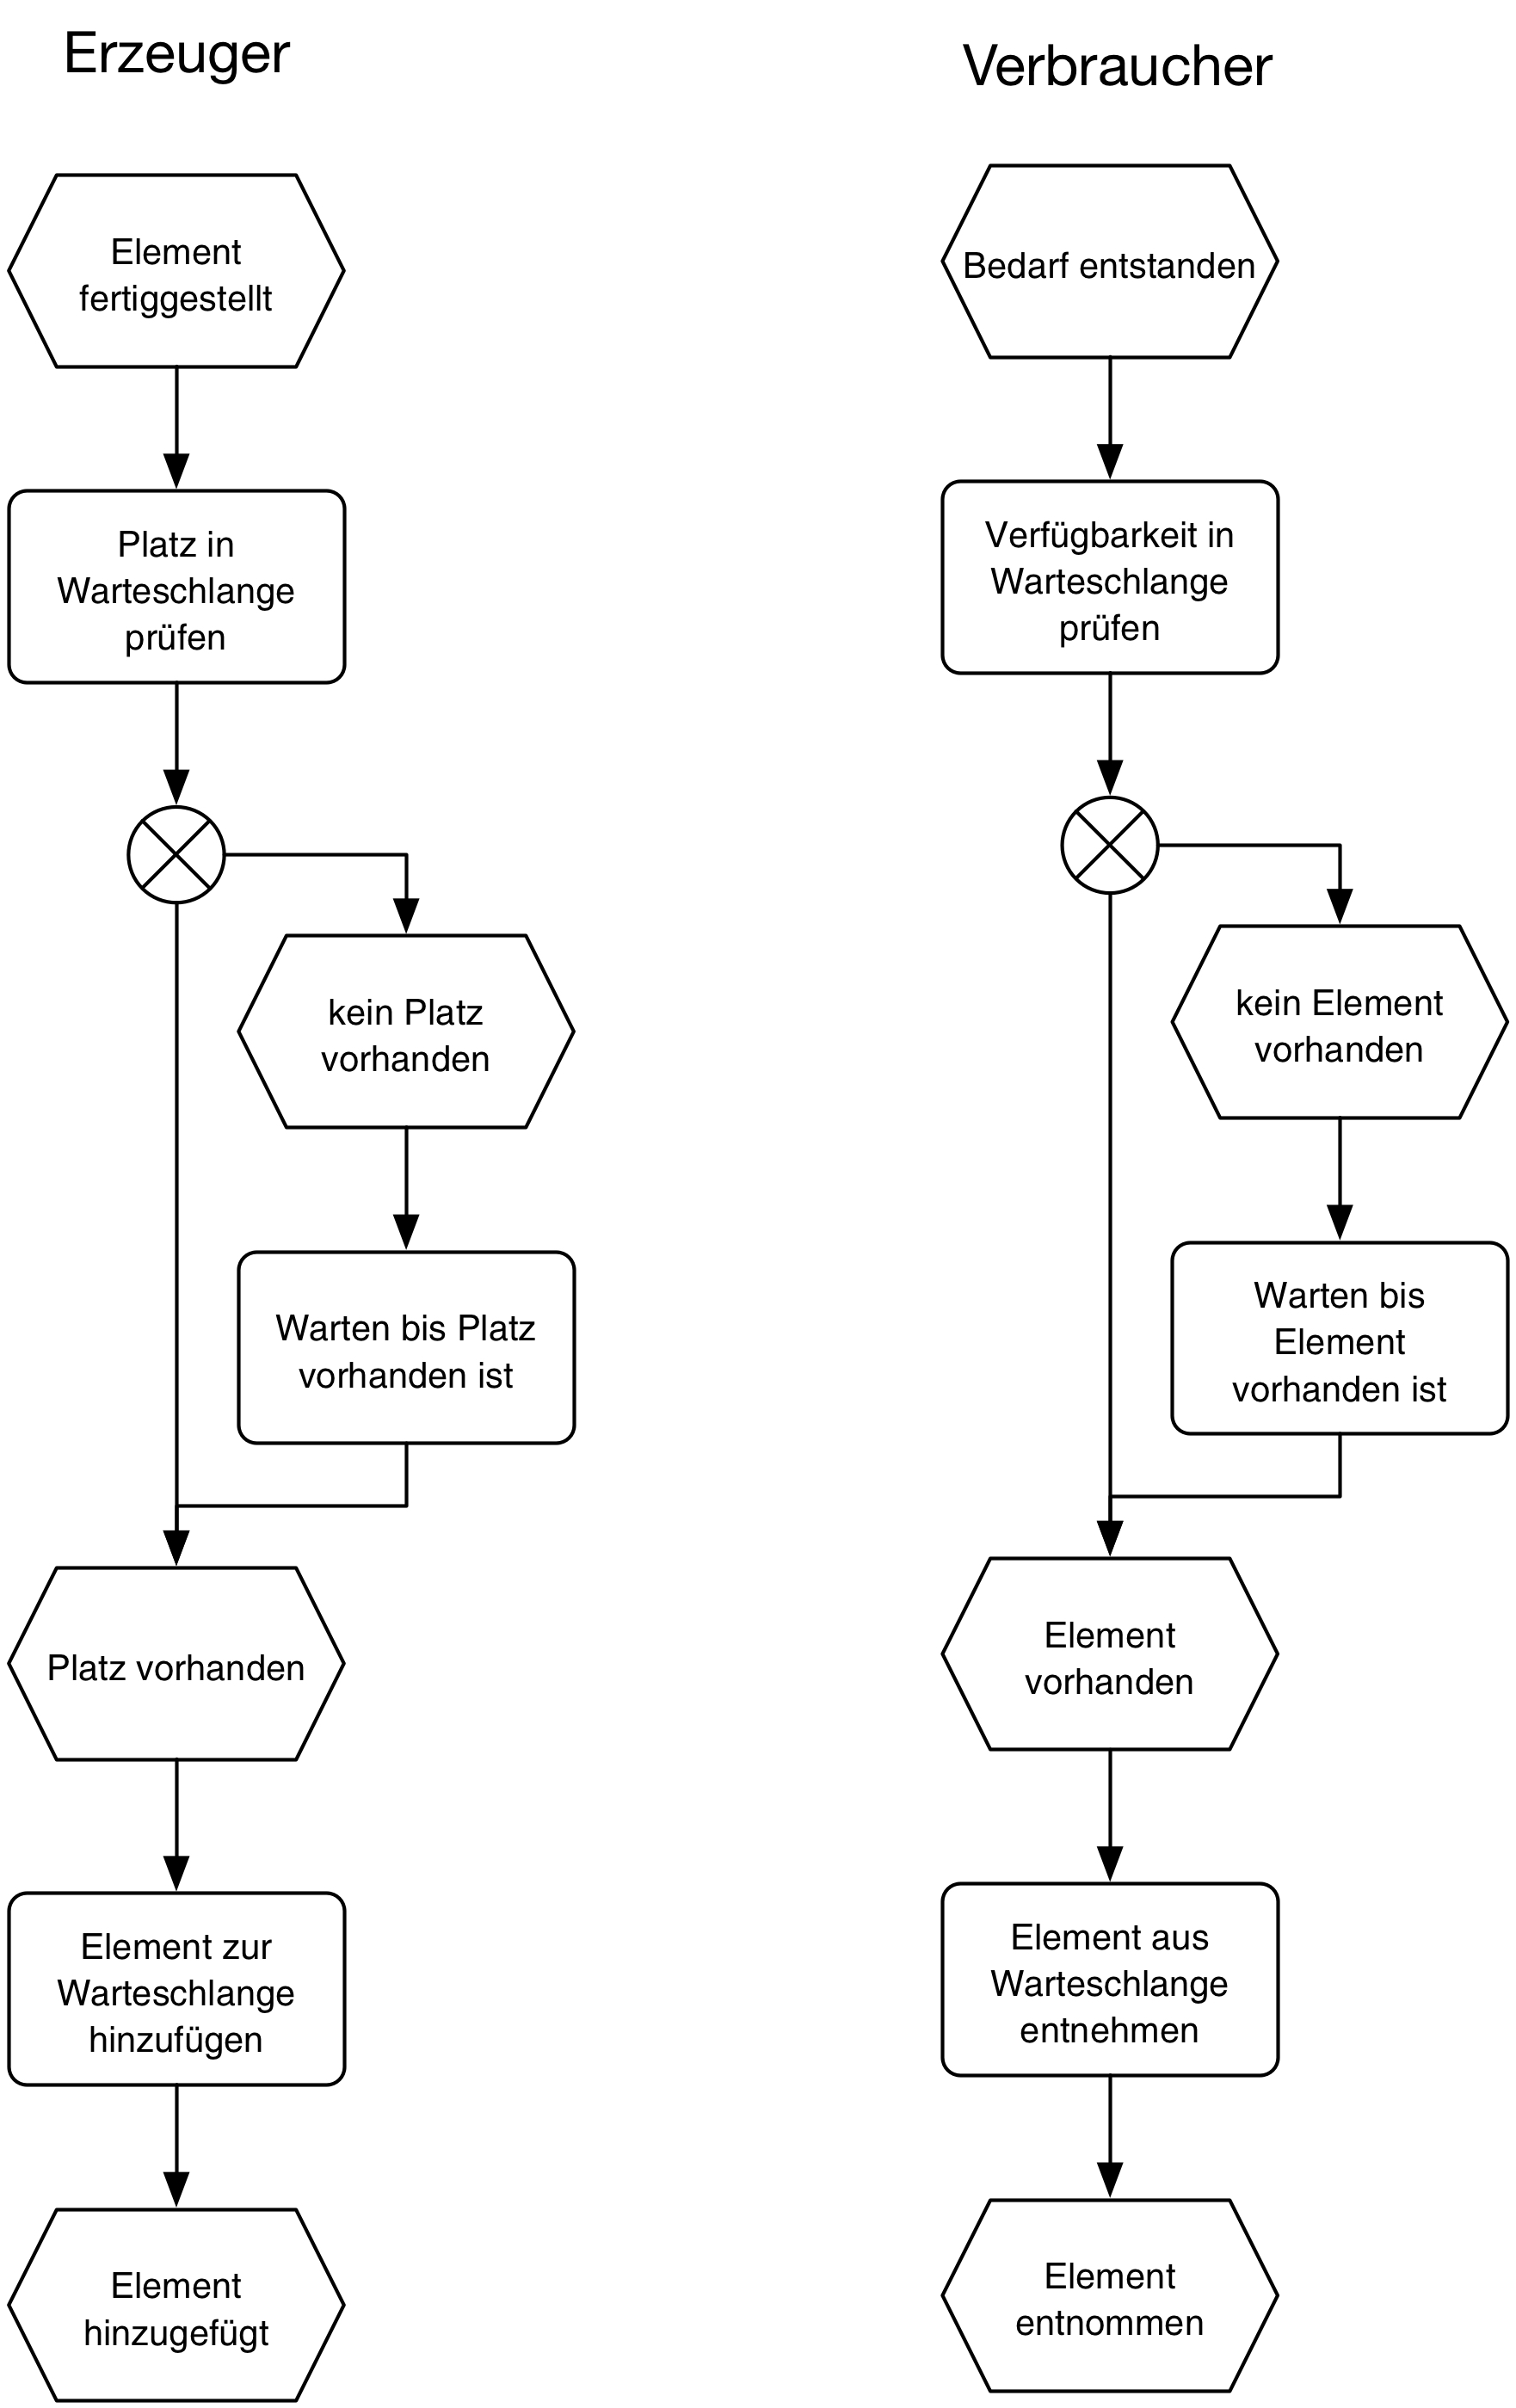
\includegraphics[width=.5\textwidth]{Erzeuger-Verbraucher-EPK.jpg}
\caption{Ereignisgesteuerte Prozessketten}
\label{fig:epk}
\end{center}
\end{figure}

% subsection ereignisgesteuerte_prozessketten (end)

\subsection{UML–Diagramm} % (fold)

In Abbildung~\ref{fig:epk} sind die zur Implementierung benötigten Klassen sowie deren Beziehungen untereinander als UML–Diagramm dargestellt. Die entsprechenden Erläuterungen finden sich in Kapitel~\myref{sec:implementierung}.

\label{sub:uml_diagramm}
\begin{figure}[H]
\begin{center}
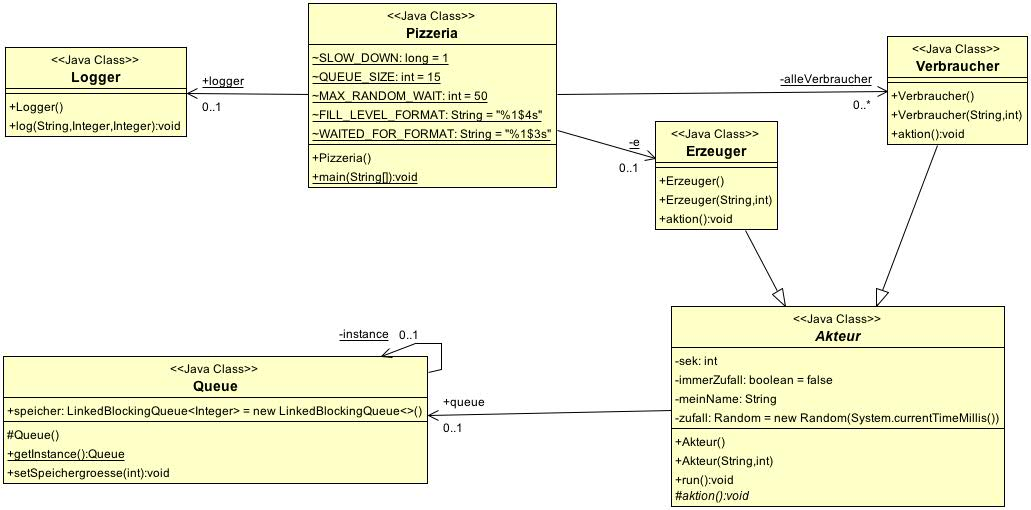
\includegraphics[width=\textwidth]{UML.jpg}
\caption{UML–Diagramm}
\label{fig:epk}
\end{center}
\end{figure}
% subsection uml_diagramm (end)

% section modellierung (end)

\newpage
\section{Implementierung} % (fold)
\label{sec:implementierung}

\subsection{Klasse: Akteur} % (fold)
\label{sub:klasse_akteur}
In der der abstrakten Klasse \code{Akteur} werden die Eigenschaften und Methoden zusammengefasst, die den Klassen \code{Erzeuger} und \code{Verbraucher} gemeinsam sind. Dazu gehören die Angaben zur Wartezeit \code{sek} bzw. \code{immerZufall} sowie die Bezeichnung \code{meinName}, die bei der Ausgabe dazu dienen kann, die Akteure zu unterscheiden. Diese Variablen werden von den Konstruktoren beim Erzeugen der Objekte befüllt. Des weiteren wird ein Generator für Pseude–Zufallszahlen sowie eine Referenz auf die Warteschlange benötigt.

In der Methode \code{run()}, die beim Starten des Threads aufgerufen wird, wird zunächst wie gefordert der Name und der Füllstand der Queue, ergänzt mit der Wartezeit ausgegeben. Anschließend wird die abstrakte Methode \code{aktion()} aufgerufen, welche die spezifischen Aktionen der abzuleitenden Klassen ausführt. Abschließend wird durch Aufruf der Methode \code{sleep()} der Elternklasse \code{Thread} die vorgegebene oder zufällig bestimmte Zeit gewartet.

Die Klasse \code{Akteur} implementiert keinen Zugriff auf die Queue und betritt somit keinen kritischen Abschnitt.
% subsection klasse_akteur (end)

\subsection{Klasse: Erzeuger} % (fold)
\label{sub:klasse_erzeuger}
Die von \code{Akteur} abgeleitete Klasse \code{Erzeuger} implementiert lediglich die Methode \code{aktion()}. Hierzu muss der kritische Abschnitt betreten werden. Hierin muss geprüft werden, ob Platz in der Queue vorhanden ist. Falls nicht, muss gewartet werden, bis dies der Fall ist. Wenn Platz vohanden ist, wird das produzierte Element\footnote{Hierbei handelt es sich in der Simulation um den Integerwert 1} in der Queue abgelegt. Anschließend wird der kritische Abschnitt wieder verlassen.

Diese Vorgehensweise entspricht der Implementierung der \code{put() } der Klasse \code{LinkedBlockingQueue}, welche indirekt über die Klasse \code{Queue} aufgerufen wird.\footnote{vgl. \cite{javadoc:lbqsourceput}}

Wie im Abschnitt~\myref{sub:kritische_abschnitte} ausgeführt, sind das Hinzufügen und das Entnehmen von Elementen bei \ac{FIFO} Warteschlangen getrennte kritische Abschnitte. Somit kann das Warten im Falle einer vollen Warteschlange durchgeführt werden, ohne eine Deadlock–Situation herbeizuführen.
% subsection klasse_erzeuger (end)

\subsection{Klasse: Verbraucher} % (fold)
\label{sub:klasse_verbraucher}
Die von \code{Akteur} abgeleitete Klasse \code{Verbraucher} implementiert lediglich die Methode \code{aktion()}. Hierzu muss der kritische Abschnitt betreten werden. Hierin muss geprüft werden, ob mindestens ein Element in der Queue vorhanden ist. Falls nicht, muss gewartet werden, bis dies der Fall ist. Wenn ein Element vohanden ist, wird das älteste entnommen. Anschließend wird der kritische Abschnitt wieder verlassen.

Diese Vorgehensweise entspricht der Implementierung der \code{take()} der Klasse \code{LinkedBlockingQueue} welche indirekt über die Klasse \code{Queue} aufgerufen wird.\footnote{vgl. \cite{javadoc:lbqsource}} 
% subsection klasse_verbraucher (end)

\subsection{Sonstige Programmmerkmale} % (fold)
\label{sub:sonstige_programmmerkmale}
Die Klasse \code{Queue} realisiert das Singleton–Entwurfsmuster, um ein Element der Klasse \code{LinkedBlockingQueue} der gewünschten Größe allen beteiligten Objekten und damit allen Threads zugänglich zu machen.\footnote{vgl. \cite{gof}, Seite 127ff}

Die Klasse \code{Logger} übernimmt die geforderte Ausgabe von „E“ bzw. „V” gefolgt von der Angabe der Zahl der momentan in der Warteschlange vorhandenen Elementen. Ergänzt werden diese Angaben von der Wartezeit\footnote{Hierbei ist die Wartezeit innerhalb des kritischen Abschnitts nicht berücksichtigt} und der dem Verbraucher zugewiesenen laufenden Nummer. Durch die Ausgabe des kompletten, zuvor zusammengesetzten Ausgabestrings in einem einzigen Aufruf von \code{System.out.println()} wird hier der konkurrierende Zugriff auf die gemeinsame Resource der Bildschirmausgabe threadischer geregelt.\footnote{siehe auch Abschnitt~\myref{sub:realisierung_mit_linkedblockingqueue}}

Die Klasse Pizzeria stellt das Gerüst der Anwendung dar. Hierin werden neben einigen Konstanten auch die benötigten Obkekte der Klassen \code{Logger} und \code{Erzeuger} sowie eine \code{ArrayList} für die nach dem Programmstart zu bestimmende Anzahl der Verbraucher definiert. Die Wartezeiten für die Verbraucher und den Erzeuger werden abgefragt und die Threads erzeugt und gestartet. Hierbei wird auch die vom Nutzer gewählte Konfiguration erfasst und zur Dokumentation in den Ausgabestrom geschrieben. Anschließend werden alle weiteren Schritte des Programms in den Threads ausgeführt. 
% subsection sonstige_programmmerkmale (end)
% section implementierung (end)

\newpage
\section{Laufzeitbetrachtungen} % (fold)
\label{sec:laufzeitbetrachtungen}

\subsection{Generelle Beobachtungen} % (fold)
\label{sub:generelle_beobachtungen}
Die erstellte Anwendung wurde in unterschiedlichen Konfigurationen ausgeführt. Ein der Aufgabenstellung entsprechender Programmlauf ist z.B. in der Logdatei \code{e0v0.0.0.txt} dokumentiert. Hier wurden ein Erzeuger–Thread und drei Verbraucher–Threads ausgeführt, deren Wartezeiten zufällig bestimmt wurden. Aufgrund der Zufälligen Wartezeit zwischen den Erzeugungs– bzw. den Verbrauchsvorgängen ist jedoch hier nur eingeschränkt eine systematische Beobachtung der Ergebnisse möglich. Allerdings zeigen sich auch hier schon fast alle für Szenarien dieser Art typischen Zustände der Akteure und der Queue, welche in den folgenden Abschnitten auch anhand von weiteren Programmläufen näher betrachtet werden.

Besonderes Augenmerk soll auf den Füllständen der Warteschlange liegen. Wie oft trifft ein Verbraucher auf eine leere Warteschlange, wie oft ein Erzeuger auf eine volle Warteschlange. Dies sind die Situationen, in denen die Programmausführung ins Stocken gerät. Ebenfalls wird die Anzahl der Situationen ermittelt, in denen weder Verbraucher noch Erzeuger warten mussten. Diese Situationen sind wohl in den meisten Fällen als Idealzustand anzusehen.

% subsection generelle_beobachtungen (end)

\subsection{Erzeuger schneller als Verbraucher} % (fold)
\label{sub:erzeuger_schneller_als_verbraucher}

% subsection erzeuger_schneller_als_verbraucher (end)

\subsection{Erzeuger langsamer als Verbraucher} % (fold)
\label{sub:erzeuger_langsamer_als_verbraucher}

% subsection erzeuger_langsamer_als_verbraucher (end)

\subsection{Ezeuger und Verbraucher gleich schnell} % (fold)
\label{sub:ezeuger_und_verbraucher_gleich_schnell}

% subsection ezeuger_und_verbraucher_gleich_schnell (end)

% section laufzeitbetrachtungen (end)